\documentclass{article}
\usepackage{helvet}
\usepackage{enumerate}
\usepackage{amsmath}
\usepackage{amsfonts}
\usepackage{graphicx}

\title{BertonGan: a conditional GAN for performing various tasks}
\author{ Aaron Schindler, Herbert Wright }
\date{\today}

\begin{document}

% the title page
\maketitle
\pagebreak

% the introduction/background section
\section{Introduction}

\subsection{Problem Statement}

Generative Adversarial Networks (GANs) \cite{goodfellow2020generative} tend to require a lot of data. We
wish to construct a network that can, given a few images of an unseen face,
construct face images/deepfakes that are similar to that one, even if it has not
seen that person before. \cite{lin2020using} is an example of face swapping, but without the
few-shot learning of new faces.

Deep learning is the traditional method of generating and detecting deepfakes \cite{nguyen2022deep}.
While some computer graphics methods can be used, they lack the same ability
of deep learning architectures to capture and learn complex functions efficiently.
Because the images generated by deepfake architectures are very realistic, most
humans are not able to distinguish between real and fake images. We can
use a different (or same in some cases) models to learn the subtle differences
between real and fake images, like differences in noise or counts of pixel colors,
to effectively decide if an image is real or not.

\subsection{Generative Adversarial Networks}

Generative Adversarial Networks were introduced by Ian Goodfellow \cite{goodfellow2020generative}.


% the methods section
\section{Methods}

\subsection{BertonGan structure}

Our approach is to train an encoder-decoder while also simultaneously training the discriminator network. Both the decoder and discriminator(s) will be conditioned on a latent variable that provides all necessary facial information. The discriminator(s) will give two values corresponding to whether or not the reconstructed image is fake and if the image also corresponds to the latent variable it has been conditioned on. The four network components of our project are outlined below: \\
\begin{enumerate}
\item Face encoder network: $f_F: \mathbb{R}^{n\times W \times H} \rightarrow \mathbb{R}^{h_f}$
\begin{enumerate}
\item Input: $n$ images of the same subjects face
\item Output: A latent representation of the subjects face
\end{enumerate}
\item Image encoder network: $f_I: \mathbb{R}^{W \times H} \rightarrow \mathbb{R}^{h_I}$
\begin{enumerate}
    \item Input: An image of a subjects face
    \item Output: A latent representation of the image
\end{enumerate}
\item Image decoder network: $f_G: \mathbb{R}^{h_F + h_I} \rightarrow \mathbb{R}^{W \times H}$
\begin{enumerate}
    \item Input: Latent representations of a face and image
    \item Output: A reconstructed image decoded from the latent features
\end{enumerate}
\item Discriminator network: $f_D: \mathbb{R}^{W \times H} \times \mathbb{R}^{h_F} \rightarrow [0,1]^2$
\begin{enumerate}
    \item Input: An image and a latent representation of a face
    \item Output: Two probabilities
    \begin{enumerate}
        \item Probability of being a fake image
        \item Probability of being a different person than the faces encoded into the latent vector
    \end{enumerate}
\end{enumerate}
\end{enumerate}
A visual encoding of the networks described above is given below:
\begin{figure}
    \centering
    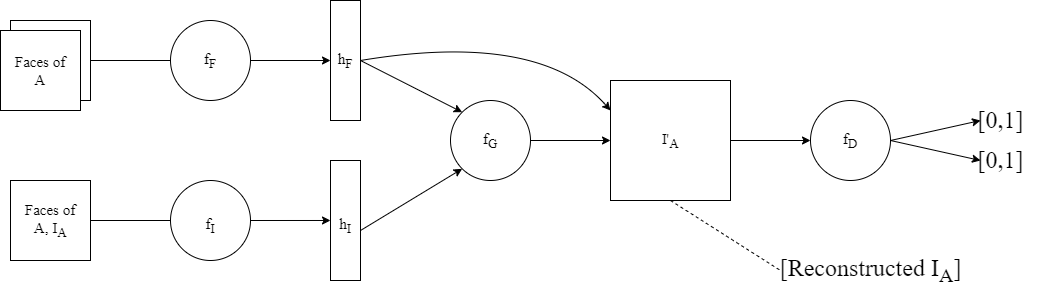
\includegraphics[scale=0.25]{images/OurNetwork.png}
    \caption{Figure 1 is a visual representation of our total network, comprising each of the four components above}
    \label{fig:my_label}
\end{figure}

\subsection{Networks}

\subsection{Training Procedure}

We propose using two datasets to train/test. The first is the built in MNIST dataset from the torchvision package. This dataset will allow us to experiment with our networks on a smaller scale, as the MNIST images are $28 \times 28$ images of numbers rather than people. The next step is to use the celebA dataset which is also built in to the torchvision package. Our original plan to use the MS-Celeb-1M dataset \cite{guo2016ms} has been changed because the dataset is no longer publicly available. The celebA dataset comprises over $200,000$ images of faces, that are \textbf{[INSERT IMAGE SIZE HERE]} in size.

Given a batch $\beta = (F_A, I_A, I_B)$, where $F_A = n$ faces of person $A$, $I_A = N$ other faces of person $A$, and $I_B = N $ faces of people other than person $A$, we will compute the following quantities:
\begin{enumerate}
    \item $h_F = f_F(F_A) \in \mathbb{R}^{h_F}$
    \item $h_I = f_I(F_B) \in \mathbb{R}^{N \times h_I}$
    \item $h_B = f_I(F_B) \in \mathbb{R}^{N \times h_I}$
    \item $I'_A = f_G(h_F, h_I) \in \mathbb{R}^{N \times W \times H}$
    \item $I'_B = f_G(h_F, h_B) \in \mathbb{R}^{N \times W \times H}$
    \item $(R_{A'}, C_{A'}) = f_D(I'_A, h_f) \in [0,1]^{N \times 2}$
    \item $(R_A, C_A) = f_D(I_A, h_F) \in [0,1]^{N \times 2}$
    \item $(R_{B'}, C_{B'}) = f_D(I'_B, h_F) \in [0,1]^{N \times 2}$
    \item $(R_B, C_B) = f_D(I_B, h_f) \in [0,1]^{N \times 2}$
    \item $D_A = \|I_A - I'_A\|$
    \item $D_B = \|I_B - I'_B\|$
\end{enumerate}

We will optimize $f_D$ by maximizing $R_A, R_B, C_A$ and minimizing $R_{A'}, R_{B'}, C_B$. We also optimize $f_F$ by maximizing $C_A, C_{A'}, C_{B'}$ and minimizing $C_B, D_A$. Additionally, we optimize $f_G, f_I$ by maximizing $R_{A'}, R_{B'}, C_{A'}, C_{B'}$ and minimizing $D_A, D_B$. All parameters are optimized by using stochastic gradient descent. 

After training, we will be able to use $f_F, f_I, \text{ and } f_G$ to perform face swaps. We will then use $f_D$ to identify fake/real images generated using face encoding $h_F$. Additionally, we will use $f_F \text{ and } f_G$ to generate new images of an already learned face.

% the experiments section
\section{Experiments}

\subsection{MNIST Experiments}

\subsection{CelebA Experiments}

% the conclusion/future work section
\section{Conclusion}

\pagebreak
% \section*{References}

\bibliography{sources}
\bibliographystyle{ieeetr}

\end{document}
